
\lstdefinestyle{bashstyle}{
    language=bash,
    basicstyle=\small\ttfamily,
    backgroundcolor=\color{gray!10},
    keywordstyle=\color{blue},
    commentstyle=\color{green!50!black},
    stringstyle=\color{red},
    showstringspaces=false,
    morekeywords={mkdir, ls, cd, mv, rm, chmod, sudo}
}

\lstdefinestyle{yaml}{
     basicstyle=\color{red}\footnotesize,
     rulecolor=\color{black},
     string=[s]{'}{'},
     stringstyle=\color{red},
     comment=[l]{:},
     commentstyle=\color{black},
     morecomment=[l]{-}
 }

\chapter{Correzione, sviluppo e ottimizzazione Demo A} \label{ch:DemoA}

All'interno di questo capitolo sarà fornita una descrizione completa dei lavori svolti nel primo progetto di demo che è stato preso in analisi inizialmente, corretto e migliorato successivamente.
\\ Inizialmente viene descritta con una breve introduzione gli obiettivi che ci si aspettava di raggiungere con lo sviluppo della demo, i problemi presenti all'inizio del lavoro svolto e le soluzioni possibili attuabili.
\\ Nella seconda parte viene trattato, entrando più nello specifico, l'implementazioni delle soluzioni proposte e presentato il lavoro finale. 
\\ Nell'ultima parte del capitolo viene infine mostrato una prova di correttezza della demo con la verifica dei suoi output e delle sue funzionalità.


\section{Introduzione alla Demo}
Come descritto al Capitolo[\ref{ch:verefoo}] Verefoo è un framework in grado di definire dei requisiti di sicurezza ad alto livello, allocare in maniera ottimale varie Network Security Functions (NSF) all'interno della topologia di rete fornita in input e configurare automaticamente tali funzioni 
automaticamente. Allo stato attuale il framework è ancora in fase di sviluppo e, nonostante si ponga gli obiettivi appena descritti, non tutte le funzionalità sono attualmente possibili all'interno del framework. Più precisamente, varie versioni del framework sono presenti in stato di sviluppo, e ognuna si occupa di allocare una possibile NSF separatamente alle altre.
All'interno di questo capitolo verrà presa in considerazione per il lavoro una di queste possibili versioni, ovvero quella che si occupa della verifica dei Network Security Requirements di protezione, dell'allocazione del numero minimo ottimale di VPN Gateway per rispettare i requisiti in input, e della configurazione di questi ultimi.\\
L'obiettivo principale di questo lavoro di demo è quindi mostrare all'utente come questa versione sia in grado, data una topologia di rete simile a quelle di una azienda di medie dimensioni, di verificare i requisiti, allocare le VPN e configurarle correttamente.
\newpage
Un altro elemento emerso durante i lavori sullo sviluppo di questa demo è stata la difficile accessibilità di quest'ultima. Per far funzionare sia il framework che la demo sono infatti necessari numerosi tool da installare all'interno della macchina in alcune versioni specifiche e potrebbe essere non immediato installare correttamente il dispositivo per far funzionare 
framework e demo. Di conseguenza come obiettivo secondario, ma di uguale importanza è stato prodotto un installer che permette all'utente di ottenere automaticamente tutti i programmi nelle versioni corrette per poter utilizzare il framework a proprio piacimento.
\\
Per portare a termine questi due obiettivi ci si è quindi interfacciati con un progetto di demo che risultava incompleto e di conseguenza non operativo. Analizzando più approfonditamente possiamo dividere le modifiche effettuate all'interno di questa demo nei seguenti punti:

\begin{enumerate}
    \item \textbf{Versione Framework}: Il file del framework iniziale era malfunzionante, in quanto ogni qual volta che si provava ad avviarlo il terminale segnalava il file come corrotto ed inutilizzabile.
    \item \textbf{Chiamate API}: La demo utilizzava delle chiamate API considerabili obsolete, di conseguenza qualsiasi relazione con il framework non produceva alcun risultato.
    \item \textbf{Installer}: Come accennato precedentemente la mancanza di un installer della Demo rendeva il framework poco accessibile e di difficile installazione manuale.
    \item \textbf{Certificati VPN}: Alcuni dei certificati di chiavi pubbliche e private erano ormai scaduti, sono quindi stati sostituiti ed i file di configurazione modificati opportunatamente.
    \item \textbf{Docker Compose}: Il file di configurazione dell'ambiente virtuale di Docker Compose conteneva errori e molti dei container non venivano istanziati correttamente.
    \item \textbf{Forwarding Rules}: Alcune forwarding rules all'interno dell'ambiente virtuale erano scorrette, sono state quindi corrette ed aggiornate per garantire la comunicazione fra tutti i nodi della rete.
\end{enumerate}

    
\section{Sviluppo Installer}
\label{sec:Installer}
Come menzionato nell'elenco precedente, uno dei punti fondamentali dei lavori effettuati su questo progetto è stata la programmazione e implementazione di un installer all'interno della demo.\\
Verefoo è un framework che per funzionare necessita le seguenti specifiche:
\begin{itemize}
    \item \textbf{Linux Ubuntu 20.04 Long Term Support(LTS)} come sistema operativo della macchina ospitante il framework.
    \item \textbf{Pv} come programma per monitorare i dati mandati attraverso la pipe.
    \item \textbf{Docker Engine} come tecnologia per istanziare e gestire container virtuali.
    \item \textbf{Docker-Compose v1} come plugin di Docker per poter istanziare e gestire molteplici container utilizzando un unico file di configurazione.
    \item  \textbf{Java openjdk-1.8} per poter eseguire il framework correttamente.
    \item \textbf{Curl} come programma per poter effettuare chiamate API con il framework.
    \item \textbf{Z3 4.8.15} come programma per risolvere il problema MaxSMT che Verefoo crea durante la computazione dell'output.
\end{itemize} 

Tuttavia al fine di poter implementare tutti questi elementi tramite terminale linux non è sufficiente installare i vari packages tramite il comando
\textit{"apt-get install [packageName]"} ma è anche necessario modificare opportunatamente alcune variabili d'ambiente all'interno del sistema operativo. Inoltre molti di questi package devono essere installati con delle versioni specifiche per evitare problemi di compatibilità,
di conseguenza per l'utente può risultare ostico riuscire a reperire ed installare tutte le versioni correttamente in quanto molti software non sono aggiornati alle versioni più recenti ma bisogna ricercare la versione specifica sui github dei vari programmi, rendendo quindi il comando apt-get install inutilizzabile.
\\ \\
Di conseguenza è stato prodotto uno script bash che da questo momento in poi verrà denominato installer che si occupa di controllare se i package sono già effettivamente presenti all'interno del sistema operativo. In caso affermativo si controlla se la versione del package è quella corretta per utilizzare Verefoo, altrimenti verrà
effettuato un downgrade della versione corrente. In caso negativo il package verrà invece istanziato direttamente.
\\Di seguito vengono mostrati e commentati alcuni snippet di codice appartententi all'installer:

\begin{lstlisting}[style=bashstyle, caption={Installazione packages curl e pv}, label=lst:bash-example,numbers=left]
    #!/bin/bash
    if which pv &> /dev/null
    then
    printf "${GREEN}pv installed... OK${COLOR_RESET}\n"
    else
    printf "${BLUE}pv package not installed. I'm going to install it\n${COLOR_RESET}\n"
    sudo apt-get update
    sudo apt-get --yes install pv
    printf "${GREEN}pv installed... OK${COLOR_RESET}\n"
    fi
    if which curl &> /dev/null
    then
    printf "${GREEN}curl installed... OK${COLOR_RESET}\n"
    else
    printf "${BLUE}curl package not installed. I'm going to install it\n${COLOR_RESET}\n"
    sudo apt-get update
    sudo apt-get --yes install curl
    printf "${GREEN}curl installed... OK${COLOR_RESET}\n"
    fi
\end{lstlisting}

Per quanto riguarda i package pv e curl l'installazione è piuttosto semplice, infatti si può notare come sia alla riga 2 che alla riga 11 venga controllato che i comandi pv e curl siano presenti reinderizzando l'output sia in caso di successo che di errore al folder /dev/null che è un folder nel quale i 
dati vengono cancellati automaticamente ma che restuituisce il successo o il fallimento dell'operazione. Nel caso l'operazione restituisca successo vuol dire che il package è già presente all'interno del sistema operativo, in caso contrario viene installato eseguendo precedentemente una \textit{apt-get update}
per scaricare localmente la versione più aggiornata del package.
Per quanto riguarda l'installazione di java invece l'installazione è leggermente più complessa:

\begin{lstlisting}[style=bashstyle, caption={Installazione java openjdk}, label=lst:bash-example,numbers=left]
    VERSION=$(java -version 2>&1 >/dev/null | grep "java version\|openjdk version")
    if [ "" = "$VERSION" ]; then
    printf "${BLUE}Java-openjdk not installed. I'm going to install it\n${COLOR_RESET}\n"
    sudo apt-get update
    sudo apt-get --yes install openjdk-8-jdk 
    echo "JAVA_HOME=/usr/lib/jvm/java-1.8.0-openjdk-amd64/jre" | sudo tee -a /etc/environment
    printf "${GREEN}Java installed... OK${COLOR_RESET}\n"
    else
    printf "${GREEN}Java openjdk installed... OK${COLOR_RESET}\n"
    fi
\end{lstlisting}

In questo caso per controllare se la versione corretta di java sia già installata viene invocato il comando \textit{"java -version"} effettuando un redirect dell'output
e intercettando delle righe contententi le stringhe "java version" o "openjdk version" assegnando questo risultato alla variabile VERSION. \\
Successivamente viene controllato se il risultato dato da questo comando corrisponde alla stringa vuota o se effettivamente è stata trovata una versione di java.
Nel caso in cui java non sia presente all'interno del sistema operativo viene installato tramite il comando \textit{"apt-get install openjdk-8-jdk"} e infine viene definito il path dove il sistema operativo dovrà andare
a cercare le varie librerie di sistema ogni qualvolta un comando java verrà eseguito, che viene salvato all'interno del file contentente tutte le variabili d'ambiente, che si trova al path:\textit{"/etc/environment"}. 

\begin{lstlisting}[style=bashstyle, caption={Installazione Docker e Docker Compose}, label=lst:bash-example,numbers=left]
    if [ -x "$(command -v docker)" ]; then
    printf "${GREEN}docker installed... OK${COLOR_RESET}\n"
    else
     printf "${BLUE}Docker engine not installed. I'm going to install it\n${COLOR_RESET}\n"
    sudo apt-get update
    sudo apt-get install ca-certificates curl gnupg
    sudo install -m 0755 -d /etc/apt/keyrings
    curl -fsSL https://download.docker.com/linux/ubuntu/gpg | sudo gpg --dearmor -o /etc/apt/keyrings/docker.gpg
    sudo chmod a+r /etc/apt/keyrings/docker.gpg
    echo \
  "deb [arch="$(dpkg --print-architecture)" signed-by=/etc/apt/keyrings/docker.gpg] https://download.docker.com/linux/ubuntu \
  "$(. /etc/os-release && echo "$VERSION_CODENAME")" stable" | \
  sudo tee /etc/apt/sources.list.d/docker.list > /dev/null
  sudo apt-get --yes install docker-ce docker-ce-cli containerd.io docker-buildx-plugin docker-compose-plugin
    printf "${GREEN}docker engine installed installed... OK${COLOR_RESET}\n"
    fi
    if [ -x "$(command -v docker-compose)" ]; then
    printf "${GREEN}docker-compose installed... OK${COLOR_RESET}\n"
    else
    printf "${BLUE}Docker-compose package not installed. I'm going to install it\n${COLOR_RESET}\n"
    sudo apt-get update
    sudo apt-get --yes install docker-compose
    printf "${GREEN}docker-compose installed... OK${COLOR_RESET}\n"
    fi

\end{lstlisting}

In questa parte di codice viene installato Docker ed il suo plugin docker-compose. Similmente all'installazione di curl e pv 
viene controllata l'esistenza di entrambi alle righe 1 e 17 e successivamente vengono installati utilizzando la documentazione ufficiale di 
Docker\cite{dockerubuntu} e di Docker-Compose\cite{dockercomposelinux}

\begin{lstlisting}[style=bashstyle, caption={Installazione Z3}, label=lst:bash-example,numbers=left]
    FILE=/home/z3
    if [ -d "$FILE" ]; then
    printf "${GREEN}z3 exists in /home directory... OK${COLOR_RESET}\n"
    else
    printf "${BLUE}z3 doesnt exist in home directory, im going to install it\n${COLOR_RESET}\n"
    cd /home
    sudo curl -LO  https://github.com/Z3Prover/z3/releases/download/
                    z3-4.8.15/z3-4.8.15-x64-glibc-2.31.zip
    sudo unzip z3-4.8.15-x64-glibc-2.31.zip
    sudo rm z3-4.8.15-x64-glibc-2.31.zip 
    sudo mv z3-4.8.15-x64-glibc-2.31 z3    #rename z3-4.8.15 into z3 
    echo "LD_LIBRARY_PATH=$LD_LIBRARY_PATH:/home/z3/bin/" | sudo tee -a /etc/environment # Care!! >> not > or it will over write environment variables
    sudo echo "Z3=/home/z3/bin/" | sudo tee -a /etc/environment
    printf "${GREEN}Z3 installed and environment variables setted... OK${COLOR_RESET}\n"
    fi
\end{lstlisting}
Come ultimo passo l'installer controlla l'esistenza del tool di Z3 all'interno del sistema operativo. Diversamente dai packages standard installati finora, per potersi far rilevare correttamente dal framework
è necessario che Z3 sia installato nella Home directory con un path definito come \textit{"/home/z3"}. Conseguentemente per controllare l'esistenza del tool è necessario quindi verificare solo la presenza del folder z3 nella home directory.
In caso di installazione necessaria tramite una chiamata API con curl viene scaricato dal github ufficiale di Z3 \cite{z3prover} la versione desiderata di Z3, estratta nella home directory e rinominata in \textit{"z3"}.
Infine vengono istanziate 2 variabili d'ambiente ovvero \textit{"LD-LIBRARY-PATH"} e \textit{"Z3"} all'interno del file con le variabili d'ambiente che si trova al path \textit{"/etc/environment"}.

\section{Implementazione}
Il secondo e più corposo lavoro all'interno di questa prima parte della tesi è stata l'effettiva realizzazione della Demo A tramite ambiente virtuale. L'obiettivo principale che ci si è posti da raggiungere è stato di mostrare le potenzialità di Verefoo proponendo all'utente una topologia di rete 
che si avvicinasse il più possibile a quella di una rete di un'azienda di piccole dimensioni. Per raggiungere tali scopi la soluzione che è stata implementata è la seguente:

\begin{figure}[h]  % 'h' significa che la figura viene posizionata qui
    \centering
    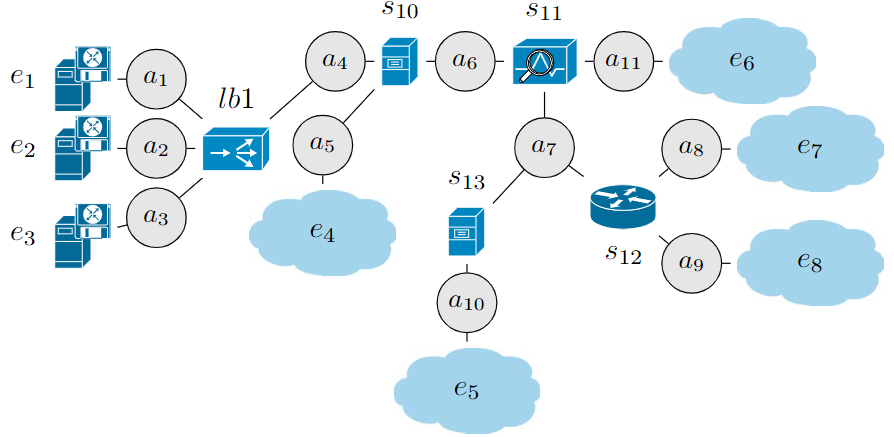
\includegraphics[width=1\textwidth]{VPN_AG.PNG} 
    \caption{Service Graph Demo A}
    \label{fig:ServiceGraph}
\end{figure}
Come è possibile notare, la topologia proposta presenta sulla sinistra 3 WebServer (e1, e2, e3) il cui traffico viene gestito da un load balancer (lb1) il quale si occupa di evitare congestioni di traffico durante le comunicazioni fra clients e servers. 
Congiuntamente ai WebServer sono presenti anche 5 endpoints (e4, e5, e6, e7, e8) che all'interno dell'ambiente virtuale verranno istanziati come fossero dei WebClients. 
Al fine di poter testare il corretto funzionamento del framework all'interno della rete sono anche presenti dei nodi che fungeranno da monitor, come il nodo  s11, ed altri che invece svolgeranno la semplice funzione di forwarder con le rispettive static routes, per simulare dei router generici. 
Infine sono presenti diversi nodi al momento vuoti che rappresentano gli  allocation places che Verefoo richiede fra i suoi possibili input per velocizzare il processo di risoluzione del problema MaxSMT. All'interno di questi nodi, il framework potrà collocare delle network security functions per assicurarsi 
il corretto funzionamento dei requisiti di sicurezza all'interno della rete.\\ Di seguito viene fornita una tabella con la definizione di ogni nodo, del suo indirizzo IP che verrà utilizzato nell'ambiente virtuale e della sua funzionalità all'interno della topologia. \\

\begin{table}
    \centering
    \begin{tabular}{ccc}
        \hline
         Name & IP & Functionality \\
        \hline
        e1 & 130.10.0.1 & Web servers behind load balancer b1 \\
        e2 & 130.10.0.2 & * \\
        e3 & 130.10.0.3 & * \\
        e4 & 40.40.41.1 & Web Client \\ 
        e5 & 40.40.42.1 & Web Client \\
        e6 & 88.80.84.1 & Web Client \\
        e7 & 192.168.1.1 & Web Client \\
        e8 & 192.168.2.1 & Web Client \\
        lb1 & 130.10.0.4 & Load Balancer \\
        s10 & 33.33.33.2 & Web Cache \\
        s11 & 33.33.33.3 & Forwarder \\
        s12 & 220.124.30.1 & Forwarder \\
        s13 & 33.33.33.4 & Forwarder \\
        a7 & 1.0.0.7 & Forwarder \\
        \hline
    \end{tabular}
    \caption{Node definitions and functionalities}
    \label{tab:tabella}
\end{table}


Oltre alla definizione del Service Graph per la demo è necessario fornire al framework anche l'insieme di security requirement che la rete deve avere, ovvero una traduzione di tutte le prioprietà di sicurezza che vorremmo fossero presenti all'interno della nostra azienda.\\
Per poter simulare il più possibile un'azienda reale è stato stabilito di creare numerosi requisiti di protezione con l'obiettivo di avere una topologia di output che contenesse un numero elevato di VPN Gateway (6), in quanto è molto comune anche in ambienti di smart working avere dei tunnel dedicati per ogni Host che lavora all'esterno della rete aziendale.. 
Al fine di poter ottenere una topologia simile sono state definite le seguenti regole:\\


\begin{table}[H]
    \centering
    \small
    \setlength{\tabcolsep}{1pt} % Riduci il padding delle colonne
    \begin{tabular}{ccccccccc}
        \hline
         Policy & IPSrc & IPDst & pSrc & pDst & tProto & Confidentiality & Intregrity & Untrusted nodes\\
        \hline
        Protection & 40.40.41.1 & 130.10.0.1 & * & 22 & ANY & AES-256-CBC & SHA2-256 & 33.33.33.2 \\
        Protection & 88.80.84.1 & 130.10.0.* & * & 80 & ANY & AES-256-CBC & SHA2-256 & 33.33.33.2/33.33.33.3 \\
        Protection & 192.168.1.1 & 130.10.0.1 & * & * & ANY & AES-256-CBC & SHA2-256 & 33.33.33.2/33.33.33.3 \\
        Protection & 40.40.42.1 & 192.168.2.1 & * & * & ANY & AES-256-CBC & SHA2-256 & 33.33.33.4/220.124.30.1 \\
        \hline
    \end{tabular}
    \caption{Security Requirements Definition DemoA}
    \label{tab:tabella}
\end{table}
\begin{itemize}
    \item \textbf{Prima Regola}: Il Web Client e4 deve poter comunicare in maniera sicura con il Web Server e1. Il traffico originato da e4 può utilizzare qualsiasi porta di uscita per il protocollo di trasporto ma il Server e1 deve ricevere i dati in ingresso unicamente dalla porta 22. È possibile utilizzare sia il protocollo UDP che TCP per il trasporto. Viene specificato infine il nodo s10 come nodo non sicuro e attraverso il quale il traffico deve passare cifrato.
    \item \textbf{Seconda regola}: Il Web Client e6 deve poter comunicare in maniera sicura con tutti i Web Server (e1, e2, e3). Il traffico originato da e6 può utilizzare qualsiasi porta di uscita per il protocollo di trasporto ma i Server devono ricevere i dati in ingresso solo dalla porta 80. È possibile utilizzare sia il protocollo UDP che TCP per il trasporto. In questo caso i nodi considerati non sicuri sono s10 e s11.
    \item \textbf{Terza Regola}: Il Web Client e7 deve poter comunicare in maniera sicura con il Web Server e1. Non ci sono limitazioni sulle porte per il traffico in entrata ed in uscita e può essere utilizzato qualsiasi protocollo di quarto livello per il trasporto. I nodi non sicuri, come per la seconda regola, sono s10 e s11. 
    \item \textbf{Quarta Regola}: Il Web Client e5 deve poter comunicare in maniera sicura con il Web Client e8. Come per la terza regola, non ci sono limitazioni sulle porte e protocollo di trasporto da utilizzare. I nodi considerati non sicuri per questa regola sono s12 ed s13.
\end{itemize}

Definire questi elementi all'interno del framework di Verefoo non è comunque sufficiente per creare una demo, in quanto come già visto al Capitolo[\ref{ch:verefoo}] è sufficiente descrivere in file XML la definizione dei nodi ed i corrispettivi indirizzi ip e nodi adiacenti. \\
Per avere una demo che invece dimostri la correttezza delle operazioni del framework è necessario istanziare gli elementi descritti in output e successivamente tradurli in un ambiente virtuale di container Docker. Di seguito è quindi disponibile la definizione di alcuni services
per la topologia descritta in precedenza:

\begin{lstlisting}[style=yaml,caption={Definizione di Services dell'ambiente virtuale DemoA},label=composeDemoA]
    services:
        server1:
            container_name: server1
            hostname: server1
            image: endpoint
            cap_add:
            - NET_ADMIN
            command: sh -c "route del default && route add -net 0.0.0.0 netmask 0.0.0.0 gw 130.10.0.4 && tail -F anything"
            networks:
                servers:
                    ipv4_address: 130.10.0.1
    
        end4:
            container_name: end4
            hostname: end4
            image: endpoint
            cap_add:
                - NET_ADMIN
            command: sh -c "route del default && route add -net 0.0.0.0 netmask 0.0.0.0 gw 40.40.41.100 && tail -F anything"
            networks:
                endpoints4:
                    ipv4_address: 40.40.41.1
    
\end{lstlisting}

Scendendo nel dettaglio sono mostrati principalmente un server ed un endpoint, che appartengono a sottoreti differenti ma che hanno la stessa immagine di partenza nella costruzione del container.
Entrambi infatti verranno configurati come endpoint e le loro forwarding route verranno cancellate completamente, indicando come unico gateway un ip stabilito arbitrariamente nella sottorete in cui appartengono.
Inoltre tramite il cap-add viene dato a ciascun endpoint la capacità di NET-ADMIN che consente al container di configurare l'interfaccia di rete e le route.

\section{Output}
Fornendo gli input definiti precedentemente il framework cercherà una soluzione che non solo soddisfi tutte le regole, ma che impieghi anche il minor numero di risorse necessarie per garantire tali proprietà. Verefoo risolverà quindi un problema di tipo MaxSMT (Maximum Satisfiability Modulo Theories). 
Nel caso specifico di questa topologia con i requisiti di sicurezza previamente definiti nel paragrafo precedente il risultato prodotto in output sarà il seguente:
\begin{figure}[h]  % 'h' significa che la figura viene posizionata qui
    \centering
    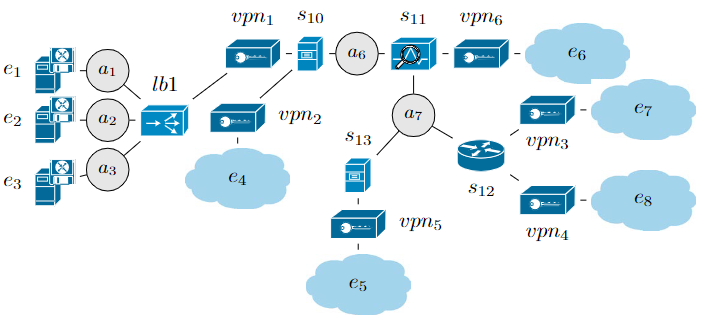
\includegraphics[width=1\textwidth]{VPN_deploy.PNG} 
    \caption{Verefoo Output Demo A}
    \label{fig:VPNDeployA}
\end{figure}

Come era prevedibile, diversi VPN Gateway sono stati allocati al posto dei vari Allocation Places definiti nell'input fornito a Verefoo. Data questa soluzione che dovrebbe essere la soluzione al problema definito prima, proveremo a testare dentro l'ambiente virtuale la funzionalità dei vari tunnel VPN, per assicurarci che il framework lavori correttamente.
Prima di procedere però è importante anche analizzare i vari elementi che Verefoo ha prodotto. Il framework infatti non ha solo allocato negli allocation places corretti i Gateway, ma ha anche fornito anche una configurazione automatica da utilizzare. Nel caso specifico la configurazione per i 6 Gateway è la seguente:\\

\begin{table}[H]
    \centering
    \begin{tabular}{ccccccc}
        \hline
         \# & Action & IPSrc & IPDst & pSrc & pDst & tProto \\
        \hline
        1 & EXIT & 192.168.1.1 & 130.10.0.1 & * & * & ANY \\
        2 & EXIT & 88.80.84.1 & 130.10.0.3 & * & 80 & ANY \\
        3 & EXIT & 40.40.41.1 & 130.10.0.1 & * & 22 & ANY \\
        4 & EXIT & 88.80.84.1 & 130.10.0.1 & * & 80 & ANY \\
        5 & EXIT & 88.80.84.1 & 130.10.0.2 & * & 80 & ANY \\
        6 & ACCESS & 130.10.0.1 & 192.168.1.1 & * & * & ANY \\
        7 & ACCESS & 130.10.0.3 & 88.80.84.1 & 80 & * & ANY \\
        8 & ACCESS & 130.10.0.1 & 40.40.41.1 & 22 & * & ANY \\
        9 & ACCESS & 130.10.0.1 & 88.80.84.1 & 80 & * & ANY \\
        10 & ACCESS & 130.10.0.2 & 88.80.84.1 & 80 & * & ANY\\
        \hline
    \end{tabular}
    \caption{VPN Gateway 1}
    \label{tab:VPN Gateway 1}
\end{table}

\begin{table}[H]
    \centering
    \begin{tabular}{ccccccc}
        \hline
         \# & Action & IPSrc & IPDst & pSrc & pDst & tProto \\
        \hline
        1 & ACCESS & 40.40.41.1 & 130.10.0.1 & * & 22 & ANY \\
        2 & EXIT & 130.10.0.1 & 40.40.41.1 & 22 & * & ANY \\
        \hline
    \end{tabular}
    \caption{VPN Gateway 2}
    \label{tab:VPN Gateway 2}
\end{table}

\begin{table}[H]
    \centering
    \begin{tabular}{ccccccc}
        \hline
         \# & Action & IPSrc & IPDst & pSrc & pDst & tProto \\
        \hline
        1 & ACCESS & 192.168.1.1 & 130.10.0.1 & * & * & ANY \\
        2 & EXIT & 130.10.0.1 & 192.168.1.1 & * & * & ANY \\
        \hline
    \end{tabular}
    \caption{VPN Gateway 3}
    \label{tab:VPN Gateway 3}
\end{table}

\begin{table}[H]
    \centering
    \begin{tabular}{ccccccc}
        \hline
         \# & Action & IPSrc & IPDst & pSrc & pDst & tProto \\
        \hline
        1 & ACCESS & 192.168.2.1 & 40.40.42.1 & * & * & ANY \\
        2 & EXIT & 40.40.42.1 & 192.168.2.1 & * & * & ANY \\
        \hline
    \end{tabular}
    \caption{VPN Gateway 4}
    \label{tab:VPN Gateway 4}
\end{table}

\begin{table}[H]
    \centering
    \begin{tabular}{ccccccc}
        \hline
         \# & Action & IPSrc & IPDst & pSrc & pDst & tProto \\
        \hline
        1 & ACCESS & 40.40.42.1 & 192.168.2.1 & * & * & ANY \\
        2 & EXIT & 192.168.2.1 & 40.40.42.1 & * & * & ANY \\
        \hline
    \end{tabular}
    \caption{VPN Gateway 5}
    \label{tab:VPN Gateway 5}
\end{table}

\begin{table}[H]
    \centering
    \begin{tabular}{ccccccc}
        \hline
         \# & Action & IPSrc & IPDst & pSrc & pDst & tProto \\
        \hline
        1 & ACCESS & 88.80.84.1 & 130.10.0.1 & * & 80 & ANY \\
        2 & ACCESS & 88.80.84.1 & 130.10.0.2 & * & 80 & ANY \\
        3 & ACCESS & 88.80.84.1 & 130.10.0.3 & * & 80 & ANY \\
        4 & EXIT & 130.10.0.1 & 88.80.84.1 & 80 & * & ANY \\
        5 & EXIT & 130.10.0.2 & 88.80.84.1 & 80 & * & ANY \\
        6 & EXIT & 130.10.0.3 & 88.80.84.1 & 80 & * & ANY \\
        \hline
    \end{tabular}
    \caption{VPN Gateway 6}
    \label{tab:VPN Gateway 6}
\end{table}

Prendendo in esempio il VPN Gateway 1 è possibile notare come Verefoo non si limita ad eseguire delle configurazioni semplici ma è in grado di produrre anche configurazioni miste, ovvero non unicamente di ingresso o di uscita dal tunnel. 
È infatti possibile notare come tutto il traffico in transito può sia cifrato in Accesso (ACCESS) al tunnel che decifrato in uscita (EXIT) al tunnel.\\
Oltre alle configurazioni dei gateway VPN, Verefoo offre, tramite un traduttore automatico, dei file di configurazione per istanziare i tunnel VPN utilizzando Strongswan.\\
A fine di esempio viene fornito il file di configurazione di Strongswan di uno dei vari gateway della topologia, che verrà utilizzato per istanziare il tunnel VPN nell'ambiente virtuale:\\


\begin{lstlisting}[language=sh]
    connections {
    site-site {
      local_addrs  = 20.0.1.1
      remote_addrs = 20.0.7.2
      local {
         auth = pubkey
         certs = VpnConfig1Cert.pem
         id = VpnConfig1.strongswan.org
      }
      remote {
         auth = pubkey
         id = VpnConfig2.strongswan.org
      }
      children {
         net-net {
            local_ts = 130.10.0.1/24            
            remote_ts = 192.168.1.1/24            
            start_action = trap|start 
            rekey_time = 5400
            rekey_bytes = 500000000
            rekey_packets = 1000000
            esp_proposals = aes256-sha2_256-modp2048
         }
      }
      version = 2
      mobike = no
      reauth_time = 10800
    }
    }
\end{lstlisting}

\section{Verifiche e Test}
Definito l'ambiente virtuale e impostato le configurazioni di Verefoo prodotte in output è necessario testare e dimostrare che il framework ha prodotto una soluzione corretta.\\
Al fine di eseguire tutte le operazioni di verifica e test in maniera più trasparente possibile è stato inserito, in aggiunta alla topologia già definite nella figura (\ref{fig:VPNDeployA})
un nodo aggiuntivo, di collegamento fra il vpn gateway 4 e l'endpoint 8. 
In questo modo, utilizzando tcpdump e analizzando le interfacce di rete sarà possibile notare in quali nodi della topologia il traffico passerà in chiaro e in quali invece verrà cifrato. 
È importante sottolineare come all'interno dell'ambiente virtuale tutti gli elementi sono stati configurati precedentemente per velocizzare le operazioni di testing, di conseguenza i vari certificati pubblici e privati sono stati già generati ed inseriti all'interno dei nodi VPN, e le route di trasmissione statiche sono state già inserite per tutta la topologia tramite il file di docker-compose.\\

All'interno di questa tesi, per semplificare le operazioni di verifica effettuate non verranno verificati tutti i requisiti di sicurezza definiti precedente ma ci si limiterà a testare la connessione fra l'endpoint e5 e l'endpoint e8.\\

Per iniziare il test di correttezza sul tunnel vpn che collega i due endpoint è necessario attivare strongswan con i certificati dei due gateway vpn, utilizzando quindi il comando \textit{"swanctl -q"} all'interno del container di vpn4 e vpn5:

\begin{figure}[h]
    \begin{minipage}{0.5\textwidth}
        \centering
        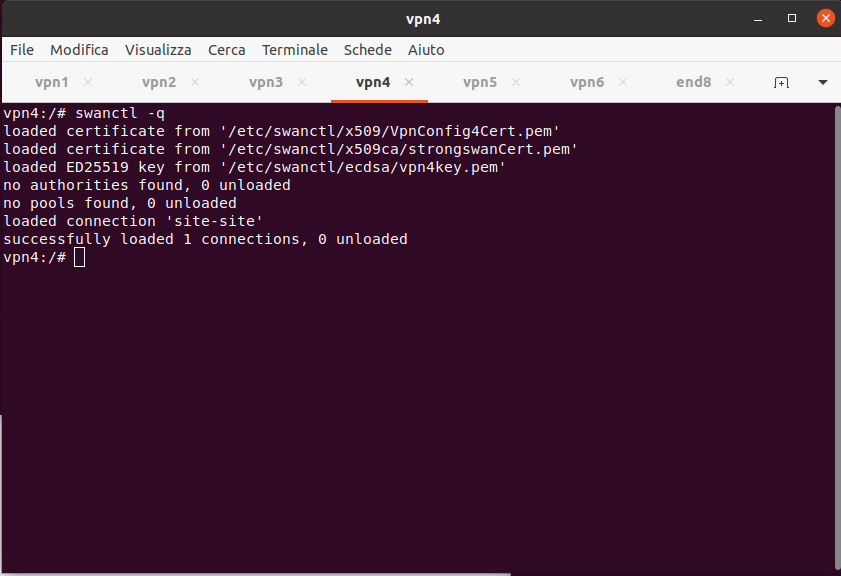
\includegraphics[width=\linewidth]{(01)FirstVPNConfig.png}
        \caption{VpnGateway4}
    \end{minipage}\hfill
    \begin{minipage}{0.5\textwidth}
        \centering
        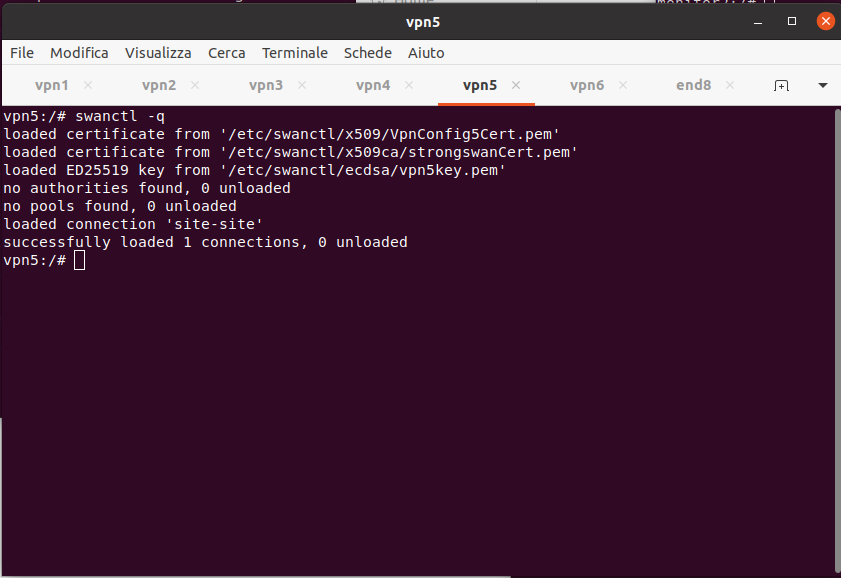
\includegraphics[width=\linewidth]{(02)SecondVPNConfig.png}
        \caption{VpnGateway5}
    \end{minipage}
\end{figure}

\newpage

Una volta caricati correttamente i vari certificati all'interno dei container, è necessario utilizzare strongswan per creare il tunnel esplicitamente. Per fare ciò è necessario invocare il seguente comando:
\textit{swanctl --initiate --child net-net}. Attraverso l'output mostrato su terminale è possibile verificare che i tunnel siano stati correttamente istanziati o se vi è stato qualche problema nello scambio dei parametri
di sicurezza.
\begin{figure}[h] 
    \centering
    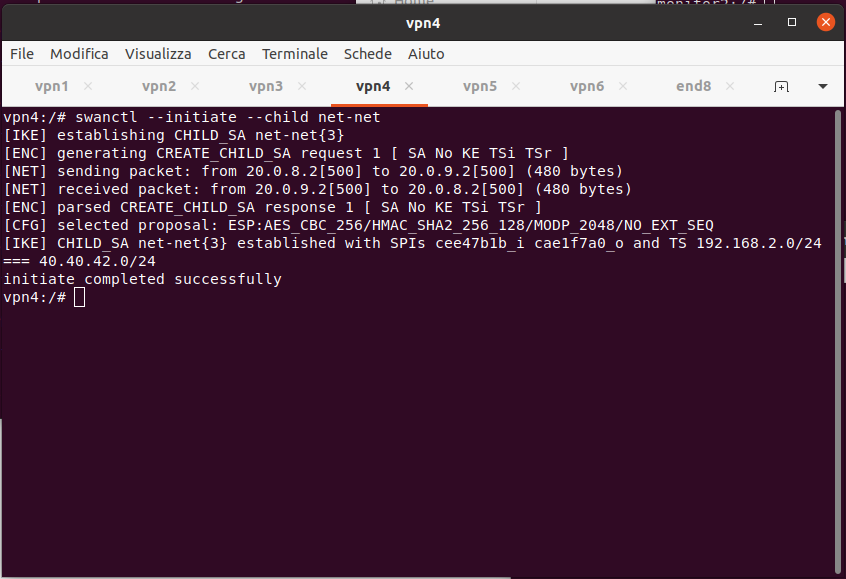
\includegraphics[width=1\textwidth]{(03)VPNConnectionEstablished.png} 
    \caption{Verifica Tunnel VPN}
    \label{fig:VPNDeploy}
\end{figure}

Come si può notare dall'output stampato sul terminale il protocollo IPsec utilizza IKE per scambiarsi le chiavi e successivamente viene stabilita la security association 
definita "net-net" nel file di configurazione swanctl. Una volta che viene stabilita la security association viene definito il traffic selector, ovvero si specifica quali pacchetti dovranno
entrare nel tunnel VPN (con rispettivo IPsrc ed IPdst). Infine vengono scelti gli algoritmi per l'autenticazione e la cifratura dei pacchetti. Se entrambi i nodi riescono ad accettare le stesse condizioni allora il tunnel viene creato.
Nel caso in esempio quindi come si può leggere nell'output il tunnel è stato configurato da Verefoo correttamente.
\\
Da questo momento in poi quindi qualsiasi pacchetto inviato dall'endpoint e8 all'endpoint e5 e viceversa verrà cifrato e non sarà possibile ispezionarlo all'interno del tunnel VPN. Per verificare ciò verranno utilizzati due monitor, 
il primo definito monitorESP sarà fornito dal container del nodo s12, mentre il secondo definito monitorICMP sarà il nodo precedentemente aggiunto fra l'endpoint e8 e il gateway vpn4. In questo modo è possibile utilizzare tcpdump e osservare le interfacce di rete nelle quali passano i pacchetti fra e8 ed e5.  
Per quanto riguarda il monitorESP la corretta interfaccia è eth1 mentre per il monitorICMP è eth0. 
Eseguiamo quindi il seguente comando: \textit{ tcpdump -i [interfacename]} su entrambi i monitor per osservare il traffico dati.

\begin{figure}[h] 
    \centering
    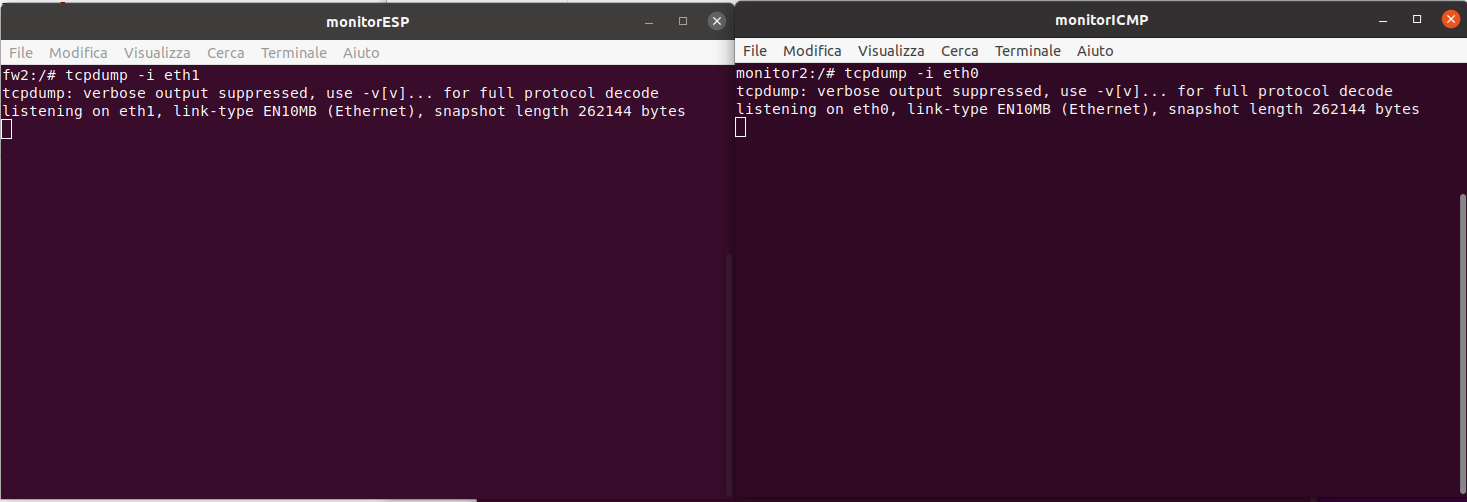
\includegraphics[width=1\textwidth]{(04)MonitorsConfig.png} 
    \caption{Tunnel stabilito}
    \label{fig:VPNDeploy}
\end{figure}

Una volta configurato tcpdump in entrambi i monitor tutti i pacchetti in transito attraverso questi due nodi verranno registrati e controllati, indicando ip e protocollo di livello 3 che viene utilizzato.
Per testare che i pacchetti vengano effettivamente cifrati correttamente quindi mandiamo dei pacchetti di ping da e8 ad e5 e controlliamo l'output dei due monitor:

\begin{figure}[H] 
    \centering
    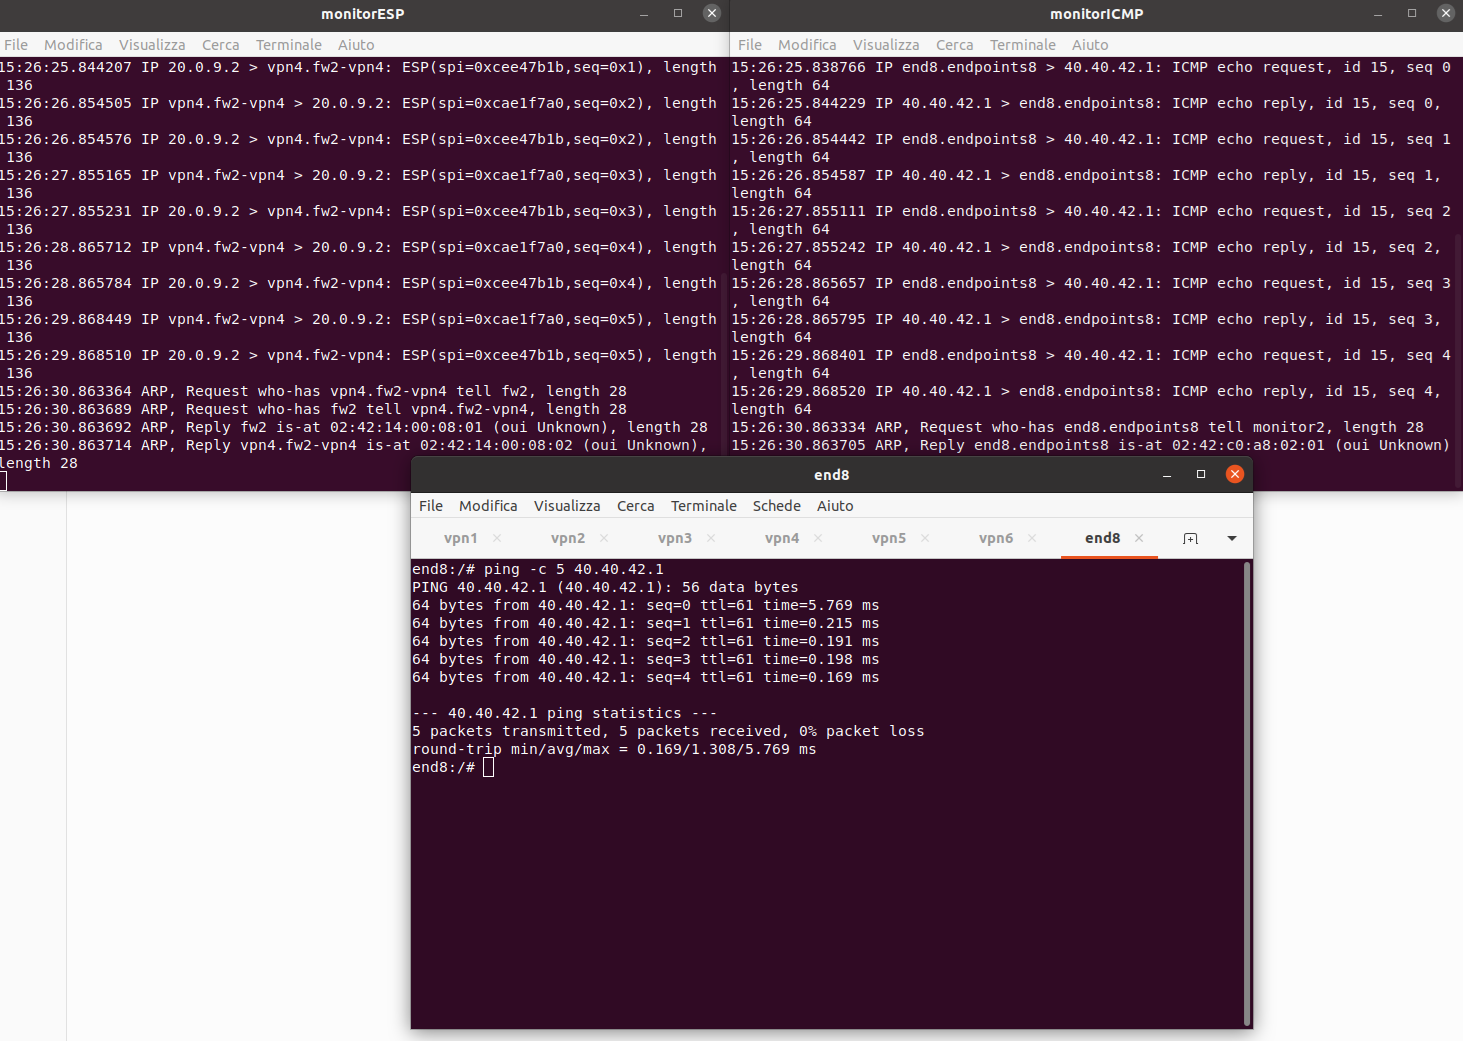
\includegraphics[width=1\textwidth]{(05)Correctness Proof.png} 
    \caption{Prova di correttezza}
    \label{fig:VPNDeploy}
\end{figure}

Osservando l'ultimo output si può dedurre che i tunnel funzionano correttamente.
Per il monitorICMP che si trova fra l'endpoint e il vpn gateway 4 il traffico viene trasmesso in chiaro ed i pacchetti vengono visualizzati come pacchetti ICMP da tcpdump, invece i pacchetti che transitano su s12 cioè dopo il passaggio dal vpn gateway vengono visualizzati come pacchetti ESP che è il protocollo utilizzato da IPsec per incapsulare i dati nei tunnel. Di conseguenza l'output prodotto da verefoo soddisfa le regole fornite ed utilizza il minor numero di risorse allocate possibili, verificando la correttezza del framework.\\
Con questo output è possibile quindi affermare il corretto funzionamento del framework e della Demo A e, di conseguenza, il raggiungimento del primo obiettivo di questo lavoro di tesi.